\section[\textit{Output Channels}]{\textit{Output Channels}}
\sectionmark{\textit{Output Channels}}
\label{sec:output_channels}

\subsection{Los parámetros del módulo}

\begin{description}
	\item[Filter] Colorea el sonido hacia grave o el agudo, a modo de combinación de un filtro paso de altos y otro paso de bajos. Solo funciona cuando está conectado hacia el exterior.
	\item[Pan] Paneo del sonido. Funciona para los puertos \textit{stereo} que combinan a los canales del 1 al 4 y del 5 al 8.
	\item[Off] Interruptor que activa y desactiva la salida del canal hacia los puertos del sintetizador. Cuando su estado es \textit{Off}, el canal puede seguir siendo utilizado a modo de \textit{bus}.
	\item[Level] Ganancia de salida del canal. Solo tiene efecto hacia los puertos del sintetizador.
\end{description}

\begin{figure}
	\centering
	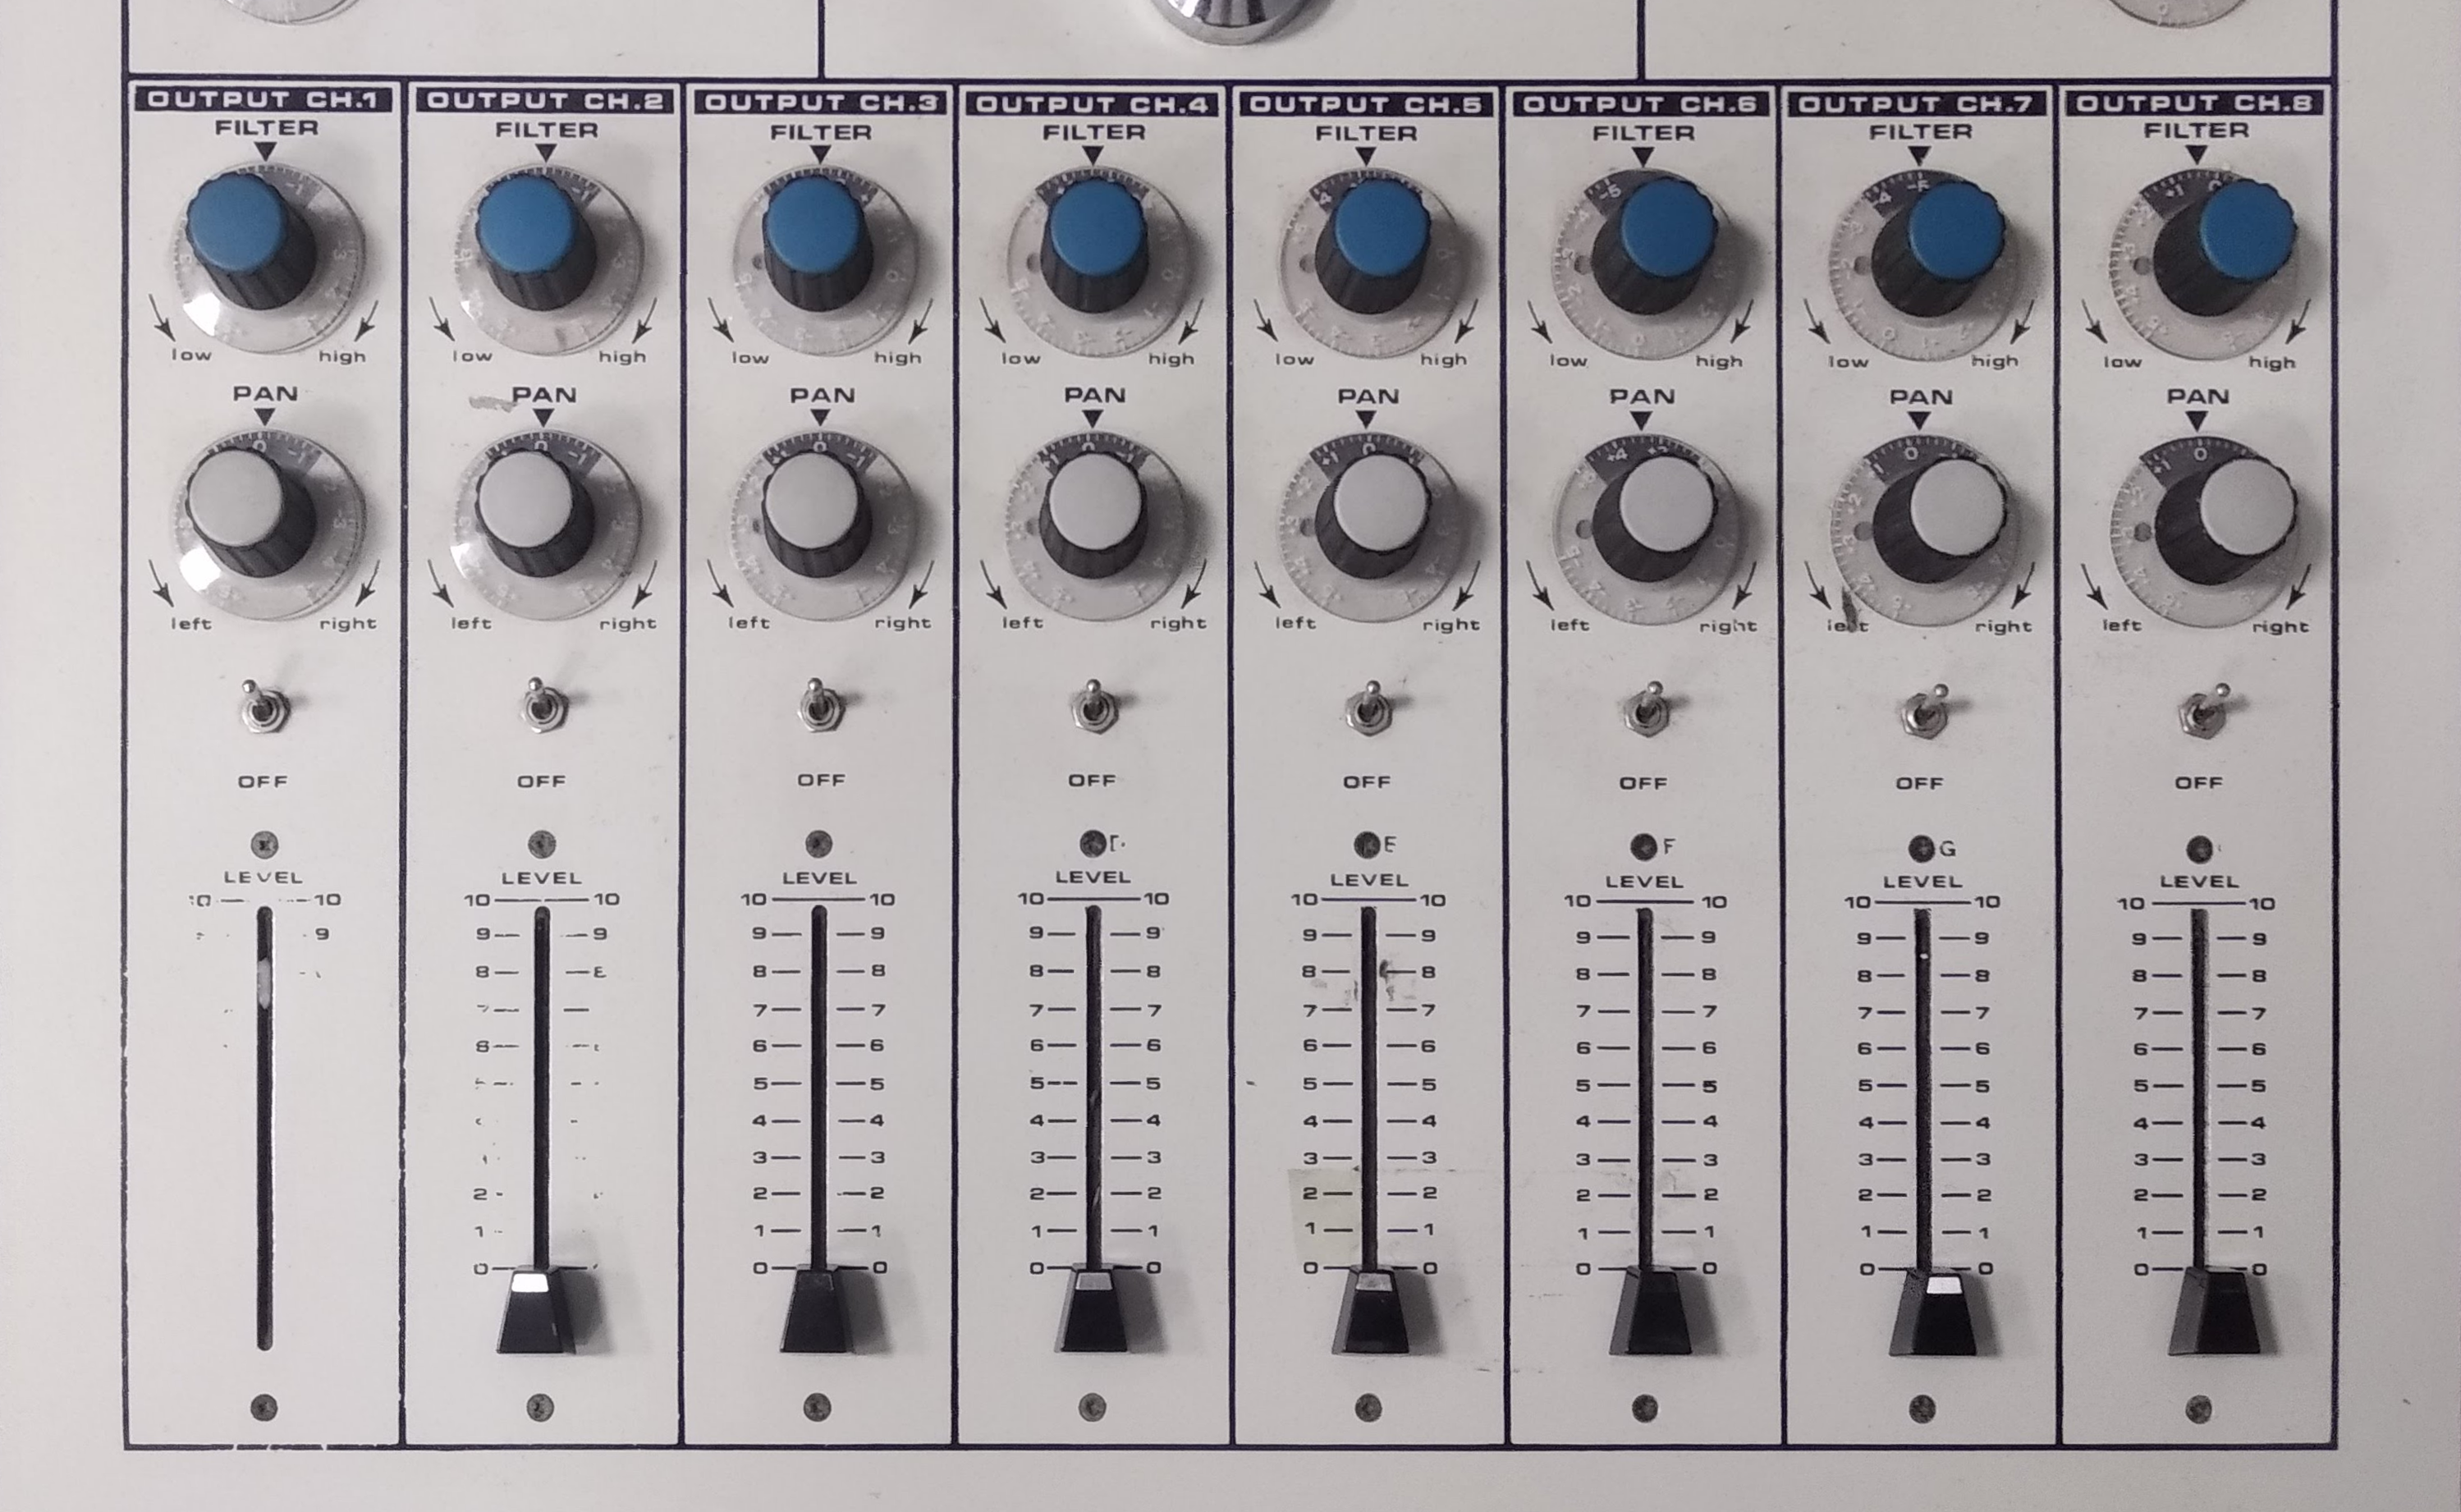
\includegraphics[width=1\textwidth]{images/output_channels}
	\caption[\textit{Output Channels}]{Vista del módulo \textit{Output Channels}, 8 canales de salida independientes. Se aprecia en la foto el estado del Synthi 100 del GME, al que le falta uno de los controles deslizantes debido al repetido uso del mismo.}
	\label{fig:output_channels}
\end{figure}

\subsection{Salidas y \textit{busses} internos}
Los 8 canales tienen como destino natural los puertos del sintetizador, bien hacia salidas stereofónicas, bien monofónicas. En todo caso, siguiendo el principio de ductilidad que lo caracteriza, estos canales pueden ser utilizados como simples \textit{busses} internos capaces de reenviar la señal de entrada a cualquier módulo, como audio y como voltaje. El interruptor \textit{Off} que incluye cada canal, permite activar o desactivar la salida a los puertos exteriores, pero su función de \textit{bus} permanece en todo momento, si bien no tienen efecto sobre él los diales o el control deslizante. Devuelve la señal tal como la ha recibido. Esta función de \textit{bus} resulta interesante para hacer que cualquier señal producida como audio sea utilizada como control de voltaje. De este modo, el \textit{patchbay} o matriz de \textit{Audio Control} puede ser comunicado con el de \textit{Voltage Control}.

\subsection{Implementación en SuperCollider}
Existen en el caso de \textit{Output Channels}, existen ciertas decisiones tomadas con más o menos arbitrariedad respecto a su comportamiento general. ¿Los controles  de ganacia, paneo o filtro afectan a la señal portada como si de un \textit{bus} se tratase, o se comporta en este caso como un simple \textit{bypass}? ¿El interruptor \textit{Off} desactiva solo la salida hacia los puertos del sintetizador o también al \textit{bus}? Estas cuestiones no tienen una respuesta evidente sin una comprobación empírica. Por lo pronto, se ha optado por tomar las decisiones que más posibilidades permitan, las cuales han sido descritas en el epígrafe anterior. 